% !TEX TS-program = pdflatex
% !TEX encoding = UTF-8 Unicode

%%% DOCUMENT DEFINITION
\documentclass[11pt, french]{article} % use larger type; default would be 10pt
\usepackage[utf8]{inputenc} % set input encoding (not needed with XeLaTeX)

%%% PAGE DIMENSIONS
\usepackage{geometry} % to change the page dimensions
\geometry{a4paper} % or letterpaper (US) or a5paper or....
\geometry{margin=1in} % for example, change the margins to 2 inches all round

%%% PACKAGES
\usepackage{graphicx} % support the \includegraphics command and options
\usepackage{booktabs} % for much better looking tables
\usepackage{array} % for better arrays (eg matrices) in maths
\usepackage{paralist} % very flexible & customisable lists (eg. enumerate/itemize, etc.)
\usepackage{verbatim} % adds environment for commenting out blocks of text & for better verbatim
\usepackage{subfig} % make it possible to include more than one captioned figure/table in a single float
\usepackage[frenchb]{babel}

% Package pour le dessin schéma bloc
\graphicspath{{../Automatique/}}
\usepackage{schemabloc}
\usepackage{amsmath}
\usepackage{tikz}
\usetikzlibrary{fit}

%%% HEADERS & FOOTERS
%\usepackage{fancyhdr} % This should be set AFTER setting up the page geometry
%\pagestyle{fancy} % options: empty , plain , fancy

% Rapport projet pluridisciplinaire
% : Xavier Galzin, Stanislas Bertrand, Romain Desille, Frédéric Meslin

\title{Projet pluridisciplinaire : sustentation magnétique}
\author{Xavier GALZIN, Stanislas BERTRAND, Romain DESILLE, Frédéric MESLIN}
\date{30/01/2012}

\begin{document}
\maketitle

\begin{center}
	\vspace{0.6in}
	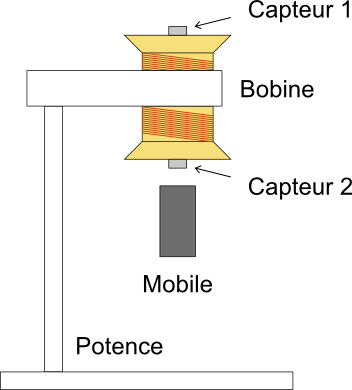
\includegraphics[width=10cm]{Automatique/system_physique.png} 
	\\
	\emph{Le système physique étudié}
\end{center}

\pagebreak

\section{Introduction}
\paragraph{}
Dans le cadre du projet pluridisciplinaire de cette année, il nous est demandé de faire léviter un mobile dans l'air à l'aide d'un champ magnétique produit par une bobine. On appelle cet effet la sustentation magnétique. Ce projet est une version édulcorée d'un prototype de lampe décorative imaginée par une étudiante de l'école LISAA (Institut supérieur des arts appliqués) et réalisée en partenariat avec des chercheurs et ingénieurs de l'INSA de Rennes.

L'étude demandée présente de nombreuses facettes : il faudra d'abord décrire et modéliser le système physique pour ensuite l'asservir à l'aide d'un dispositif automatique électronique. Ce dispositif sera réalisé de manière analogique puis de manière numérique. Dans ce rapport, nous nous intéresserons uniquement à la partie automatique, nous expliquerons la modélisation choisie ainsi que les correcteurs et leurs paramètres clefs pour faire léviter le mobile.

\section{Description du système physique}
\paragraph{}

Le système physique est existant et imposé. Il consiste en une potence munie d'une bobine qui servira à exercer le champ magnétique retenant le mobile. La bobine est également munie de capteurs à effet Hall qui permettent, par une mesure différentielle, de mesurer la distance du mobile par rapport à la bobine. Nous avons ainsi la boucle de retour de notre système. 

Nous avons donc finalement une consigne en position que nous allons convertir en un courant qui servira à générer le champ magnétique qui attirera ou repoussera le mobile et le retour en position par le biais des capteurs à effet Hall. 

Le problème principal du système est qu'il n'est pas stable en boucle ouverte. Nous allons donc procéder à une étude basée sur des mesures fournies afin de mettre en place un correcteur qui rendra la système stable. Pour cela, nous poserons les équations mathématiques du problème pour ensuite décrire le modèle de correcteur retenu ainsi que les valeurs des diverses constantes associées à ce modèle.

\section{Modélisation mathématique}

\paragraph{}
\textsc{Mise en équation du système}

\noindent
Bilan des forces appliquées sur le système :

\smallskip
$ F_{bobine/aimant}  $

$ F_{poids} = -m \times g $

$ F_{perturbations} $

...

\medskip

Devant la complexité des expressions numériques des interactions agissant sur l'OL (objet lévitant) associées à l'électromagnétisme, nous avons choisi d'étudier le problème autour du point d'équilibre (distance 15 mm) et de linéariser son fonctionnement. Nous nous étions précédemment engagés dans le calcul des constantes du modèle du second ordre via une modélisation mathématique du problème, qui nous a conduit à des résultats sans rapport avec les mesures effectuées, notamment à cause de la trop grande simplicité des expressions choisies pour la force exercée par la bobine sur l'aimant. Pour simplifier notre étude et dans le cadre de la linéarisation, on considèrera que les perturbations extérieures sur le système sont nulles. Notre stratégie est d'utiliser directement les mesures pour déterminer les constantes.


\medskip
\noindent
On applique le principe fondamental de la statique (OL immobile) :

 \medskip
$ \sum F_{exterieures}  = 0 $
 \medskip

La résolution de cette équation différentielle est complexe, l'expression de la force exercée par la bobine n'est pas linéaire et elle dépend à la fois de i et de x qui sont respectivement l'entrée et la sorties de notre système, la relation n'est pas directe. On choisit donc de linéariser (développement à l'ordre 1) l'expression de l'action de la bobine sur l'aimant autour du point d'équilibre ($I_0, X_0 $). On utilise pour cela la différentielle de la fonction.

\medskip
\noindent
Linéarisation de la force exercée par la bobine sur l'aimant :

 \medskip
$ {dF(t)}_{x = X_0, i = I_0} = \dfrac{\partial F(t)}{\partial x} \times dx + \dfrac{\partial F(t)}{\partial i} \times di $
 \medskip

\noindent
On introduit deux coefficients $ K_x $ et $ K_i $ qui correspondent respectivement aux dérivées partielles suivant x et i de F.

 \medskip
$ K_x = \dfrac{\partial F(t)}{\partial x}, K_i = \dfrac{\partial F(t)}{\partial i} $
 \medskip

\noindent
On obtient après linéarisation l'équation différentielle suivante :

 \medskip
$ F_0 - m \times g + K_x \times D_x + K_i \times D_i = 0 $
 \medskip

avec : $ D_x = x - X_0, D_i = i - I_0 $

lorsque : $ (x, i) = (X_0, I_0) \rightarrow D_x = 0, D_i = 0 \rightarrow m \times g = F_0 $

\medskip
\noindent
On applique le principe fondamental de la dynamique :

 \medskip
$ \sum F_{exterieures}  = m \times \dfrac{d^2x}{dt^2} = m \times \dfrac{d^2D_x}{dt^2} $
 \medskip

\noindent
On transfère ensuite l'équation dans le domaine de Laplace :

 \medskip
$ m \times D_x{s^2} = K_x \times D_x + K_i \times D_y $

$ D_x \times (m{s^2} - K_x) = K_i \times D_y $
 \medskip

\noindent
On obtient donc la fonction de transfert suivante :

 \medskip
$ \rightarrow H(s) = \dfrac{D_x(s)}{D_i(s)} = \dfrac{K_i}{m{s^2}- K_x}  = \dfrac{\dfrac{-K_i}{K_x}}{1 - \dfrac{m{s^2}}{K_x}} $
 \medskip

\noindent
On pose ensuite pour des raisons de simplification :

 \medskip
$ K_{meca} = \dfrac{-K_i}{K_x}, \tau_{meca} = \dfrac{m}{K_x} $

\paragraph{}
\textsc{Constantes mécaniques obtenues}

\noindent
D'après l'équation de la statique donnée précédemment :

 \medskip
$ K_x \times D_x + K_i \times D_i = 0 \rightarrow \dfrac{K_x}{K_i} = \dfrac{D_i}{D_x} $
 \medskip

\noindent
On cherche à déterminer le rapport $ \dfrac{K_x}{K_i} $ avec les mesures effectuées :

\medskip
\begin{tabular} {|l|c|c|c|}
	 \hline
	\textbf{Distance (mm)} & \textbf{Courant (A)} & \textbf{Dx (mm)} & \textbf{Di (A)} \\ \hline
	14 & 1.21 &  -1 & -0.27 \\ \hline
	15 & 1.48 & 0 & 0 \\ \hline
	16 & 1.8 & 1 & 0.32 \\ \hline
\end{tabular}

\medskip
\noindent
En faisant une régression linéaire sur la courbe, on obtient :

\medskip
$ a = \dfrac{K_x}{K_i} = 295 A.m^{-1} $

\medskip
$ b = - 2.93 A $

\medskip
$ R^2 = 0.997 $ (coefficient de détermination)
\medskip

\noindent
On peut obtenir ensuite directement la valeur de $ K_i $, on a :

\medskip
\begin{tabular} {|c|c|c|}
	 \hline
	\textbf{Dm (g)} & \textbf{Courant (A)} & \textbf{Dc (A)} \\ \hline
	0 & 1.48 &  0 \\ \hline
	10 & 1.70 & 0.22 \\ \hline
\end{tabular}

\medskip
D'où : $ K_i \approx \dfrac{Dm \times g}{Dc} = 0.446 N.A^{-1} $

\medskip
et : $ K_x = K_i \times \dfrac{K_x}{K_i} = 132 N.m ^{-1} $

\medskip
\noindent
On obtient de ces constantes les paramètres de notre modèle du deuxième ordre :

\medskip
$  K_{meca} = \dfrac {K_x}{K_i} =  295 A.m^{-1} $

\medskip
$  \tau_{meca} = \dfrac m {K_x} = 1.07 \times 10^{-3} s.rad^{-1} $

\paragraph{}
\textsc{Autres constantes du système}

\noindent
Par calcul direct, on obtient les constantes associées à la fonction de transfert de la bobine :

\medskip
$  \tau_{elec} = \dfrac L R = 6,643 \times 10^{-3} s.rad^{-1} $

\medskip
$  K_{elec} = \dfrac 1 R = 4,464 \times 10^{-1} $
\medskip

\noindent
A l'aide d'une régression linéaire effectuée sur la courbe de la tension différentielle des capteurs ($ V_{H2} - V_{H1} $) à effet Hall en fonction de la distance du mobile, on obtient :

\medskip
$  K_{hall} = 36,5 V.m^{-1} $

\medskip
$ R^2 = 0.998 $ (coefficient de détermination)
\medskip

\section{Correcteur analogique}
\subsection{Choix du correcteur}
Dans un premier temps, nous avons choisi un correcteur proportionnel-dérivé. Un correcteur dérivé n'étant pas réalisable physiquement, nous allons donc le remplacer par un correcteur à avance de phase.

\medskip
En traçant le diagramme de Black - Nichols du système non corrigé, on s'aperçoit que celui-ci est instable en boucle ouverte car en $\omega = 0$ le système est déphasé de 180\char23. Nous allons donc tenter de réduire le déphase du système afin de pouvoir passer à droite du point 0 dB, 180\char23.

\medskip
\begin{center}
\begin{tikzpicture}
\sbEntree{Vxc}
\sbComp{Comp}{Vxc}
	\sbRelier[$Vx_C$]{Vxc}{Comp}
\sbBloc{C}{$K_{p}$}{Comp}
	\sbRelier[$\epsilon_x$]{Comp}{C}
\sbBlocL{E}{$\dfrac{K_{Elec}}{\tau_{Elec} \cdot p + 1}$}{C} 
\sbBlocL{M}{$\dfrac{-\frac{K_i}{K_x}}{-{\tau_{Meca}}^2 \cdot p^2 - 1}$}{E}
\sbBlocL{H}{$K_{Hall}$}{M} 

\sbSortie{Vxr}{H} 
	\sbRelier{H}{Vxr}
	\sbNomLien[0.8]{Vxr}{$Vx_R$} 
\sbDecaleNoeudy{M}{A}
\sbBlocr[0]{A}{$\dfrac{1+ \tau_d \cdot p}{1 + a_d \cdot \tau_d \cdot p}$}{A}
\sbRelieryx{H-Vxr}{A}
\sbRelierxy{A}{Comp}
\end{tikzpicture}

$\tau_d = $


\hspace{1mm} \\ 
\hspace{1mm}\textcolor{green}{\% Paramètres du Système }\\ 
\hspace{1mm} \\ 
\hspace{1mm}\textcolor{green}{\% Modèle Electrique de la Bobine }\\ 
\hspace{1mm}R=2.24; \textcolor{green}{\%Ohm }\\ 
\hspace{1mm}L=1.49e-2; \textcolor{green}{\%H }\\ 
\hspace{1mm} \\ 
\hspace{1mm}\textcolor{green}{\% Modèle d'interaction mécanique de la bobine }\\ 
\hspace{1mm}m=0.1414; \textcolor{green}{\%Kg }\\ 
\hspace{1mm}ki=1.375; \textcolor{green}{\%N.A-1 }\\ 
\hspace{1mm}kx=117.3; \textcolor{green}{\%N.m-1 }\\ 
\hspace{1mm} \\ 
\hspace{1mm}\textcolor{green}{\% Modèle capteur effet Hall }\\ 
\hspace{1mm}Kc\_Hall=92;  \\ 
\hspace{1mm} \\ 


\emph{Schéma bloc du système complet avec correcteur}
\end{center}
\begin{quote}

%\hspace{1mm} \\ 
\hspace{1mm}\textcolor{green}{\% Paramètres du Système }\\ 
\hspace{1mm} \\ 
\hspace{1mm}\textcolor{green}{\% Modèle Electrique de la Bobine }\\ 
\hspace{1mm}R=2.24; \textcolor{green}{\%Ohm }\\ 
\hspace{1mm}L=1.49e-2; \textcolor{green}{\%H }\\ 
\hspace{1mm} \\ 
\hspace{1mm}\textcolor{green}{\% Modèle d'interaction mécanique de la bobine }\\ 
\hspace{1mm}m=0.1414; \textcolor{green}{\%Kg }\\ 
\hspace{1mm}ki=1.375; \textcolor{green}{\%N.A-1 }\\ 
\hspace{1mm}kx=117.3; \textcolor{green}{\%N.m-1 }\\ 
\hspace{1mm} \\ 
\hspace{1mm}\textcolor{green}{\% Modèle capteur effet Hall }\\ 
\hspace{1mm}Kc\_Hall=92;  \\ 
\hspace{1mm} \\ 


\end{quote}
\subsection{Choix des constantes}

Pour choisir les constantes du correcteur, nous avons procédé en deux étapes. Premièrement, nous avons réglé le correcteur à avance de phase. Pour cela, nous nous sommes servis du lieu d'Evans. On peut remarquer que, quelque soit le gain du correcteur, au moins un des pôles du système restera à droite de l'axe des imaginaires.

\begin{center}
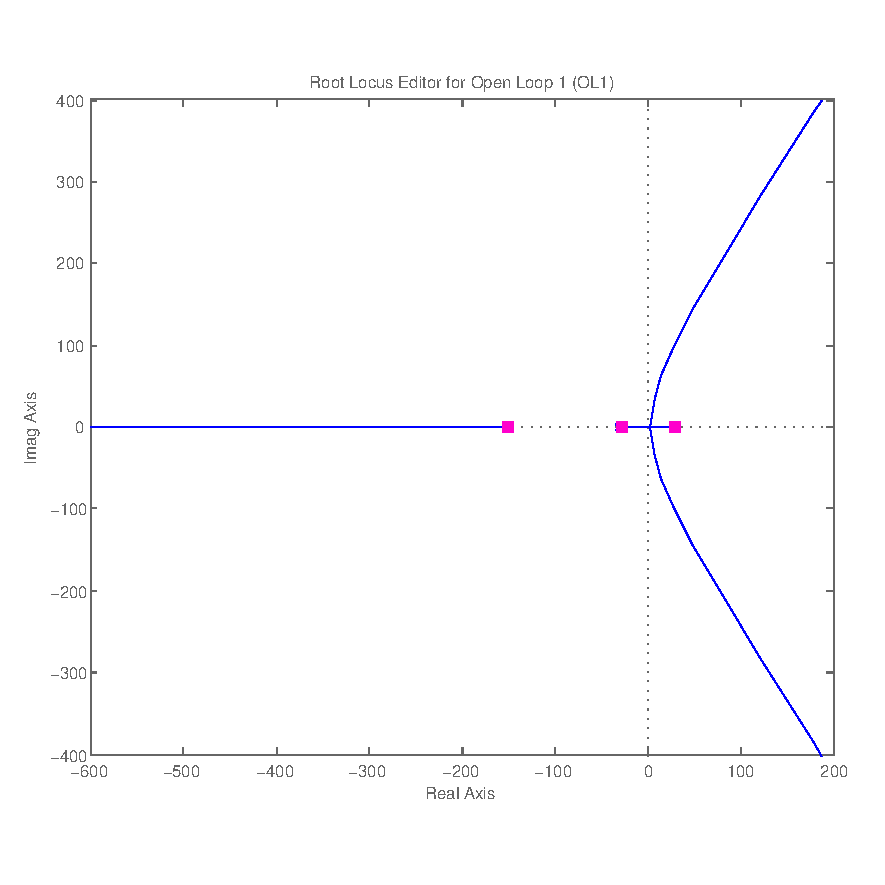
\includegraphics [scale=0.50]{RL_Sys_Seul.pdf}\\
\vspace{-10pt}
\emph{Lieu d'Evans du système non corrigé}
\end{center}

L'idée est donc de décaler le point d'intersection des asymptotes qui est normalement dans la partie droite du plan complexe en plaçant le zéros du correcteur à avance de phase dans la partie gauche tout en maintenant ce zéro entre les deux pôles issu de la constante de temps mécanique qui se trouve dans la partie gauche. On prendra le zéro du correcteur à avance de phase en $1.2*T_{m\acute{e}ca}$ afin entre les pôles mécaniques et une partie réel négative. Une fois le zéro du correcteur à avance de phase correctement placé, nous avons réglé le gain du correcteur proportionnel afin que tous les pôles du système aient une partie réelle négative. Nous avons trouvé un gain $Kp$ de 27. 

\begin{center}
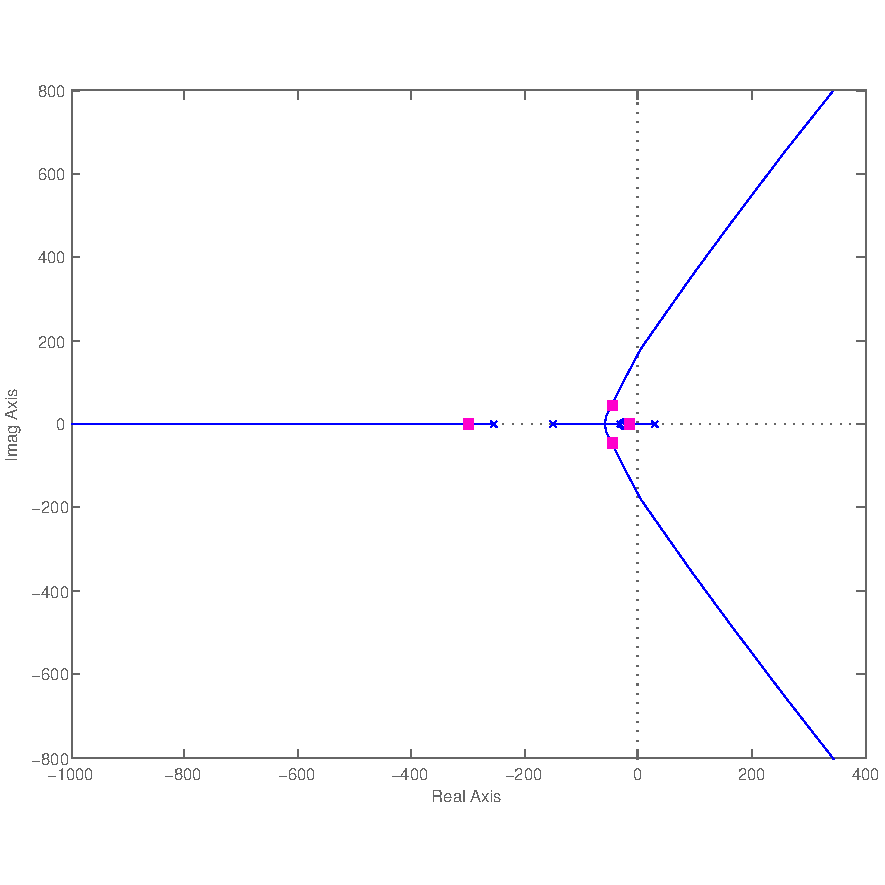
\includegraphics[scale=0.50]{RL_Sys_AvPh_K27.pdf}\\
\vspace{-15pt}
\emph{Lieu d'Evans du système corrigé}
\end{center}

Nous avons ensuite tracé le diagramme de Black - Nichols du système corrigé afin de vérifier les marges de gain et de phase. Cela nous a permis d'obtenir une marge de phase d'environ 30\char23 et une marge de gain de plus de 15 dB. Cela nous garantie une certaine immunité par rapport aux perturbations extérieures.

\begin{center}
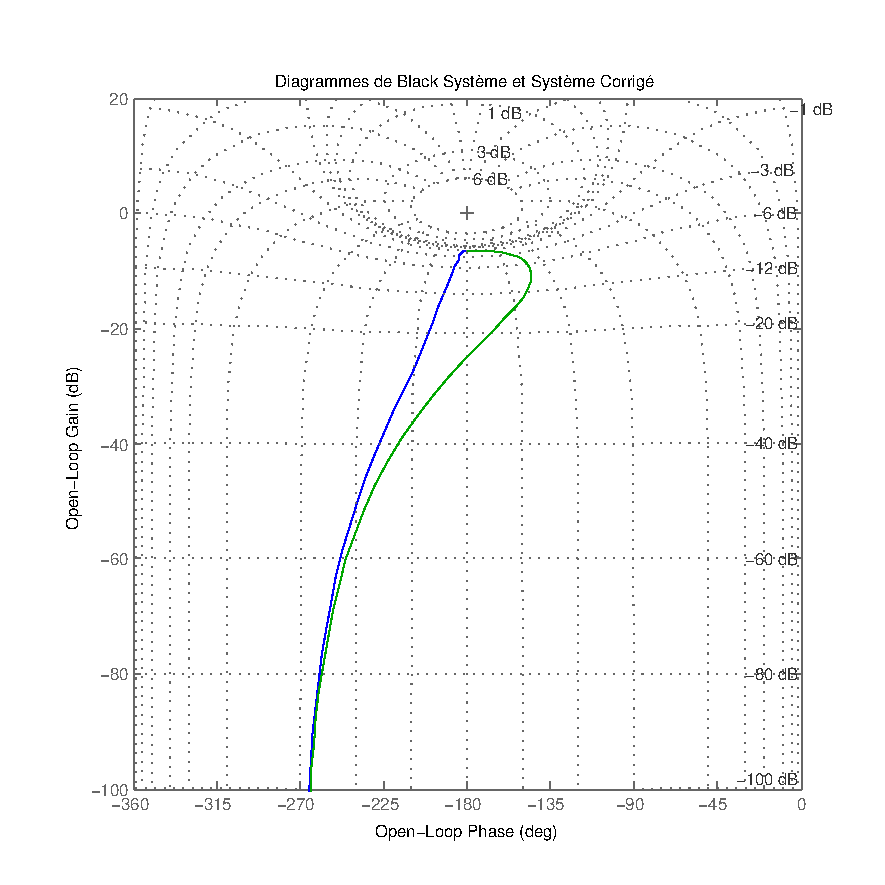
\includegraphics[scale=1]{MatBlackFredValues.pdf}

\emph{Diagramme de Black-Nichols du système corrigé}
\end{center}

\section{Correcteur numérique}

Dans la seconde partie du projet, nous commencerons par simplement convertir notre correcteur analogique par le biais d'une approximation des rectangles avant. Nous avons choisi cette solution car elle est réalisable physiquement contrairement à celle des rectangles arrière. En outre, elle est assez précise et plus facile à mettre en oeuvre que l'approximation de Tustin. Dans l'absolu, rien ne nous empêchera de changer cette approximation par la suite dans le cas où les résultats seraient insatisfaisants. 



L'équation du système par l'approximation des rectangles avant devient :
\medskip


\begin{footnotesize}
\begin{center}
$ H_{syst\grave{e}me} = \dfrac{6.379 \times 10^{-6}z^{2} + 2.393 \times 10^{-5}z + 5.596 \times 10^{-6}} {z^{3} - 2.772z^{2} + 2.542z - 0.7697} $
\hspace{2cm}
$  H_{correcteur} = \dfrac {8.272z - 7.915} {z - 0.6424} $
\end{center}
\end{footnotesize}

\begin{center}
\begin{tikzpicture}
\sbEntree{Vxc}
\sbComp{Comp}{Vxc}
	\sbRelier[$Vx_C$]{Vxc}{Comp}
\sbBloc{C}{$K_{p}$}{Comp}
	\sbRelier[$\epsilon_x$]{Comp}{C}
\sbBlocL{E}{$\dfrac{K_{Elec}}{\tau_{Elec} \cdot p + 1}$}{C} 
\sbBlocL{M}{$\dfrac{-\frac{K_i}{K_x}}{-{\tau_{Meca}}^2 \cdot p^2 - 1}$}{E}
\sbBlocL{H}{$K_{Hall}$}{M} 

\sbSortie{Vxr}{H} 
	\sbRelier{H}{Vxr}
	\sbNomLien[0.8]{Vxr}{$Vx_R$} 
\sbDecaleNoeudy{M}{A}
\sbBlocr[0]{A}{$\dfrac{1+ \tau_d \cdot p}{1 + a_d \cdot \tau_d \cdot p}$}{A}
\sbRelieryx{H-Vxr}{A}
\sbRelierxy{A}{Comp}
\end{tikzpicture}

%$\tau_d = $
%\hspace{1mm} \\ 
\hspace{1mm}\textcolor{green}{\% Paramètres du Système }\\ 
\hspace{1mm} \\ 
\hspace{1mm}\textcolor{green}{\% Modèle Electrique de la Bobine }\\ 
\hspace{1mm}R=2.24; \textcolor{green}{\%Ohm }\\ 
\hspace{1mm}L=1.49e-2; \textcolor{green}{\%H }\\ 
\hspace{1mm} \\ 
\hspace{1mm}\textcolor{green}{\% Modèle d'interaction mécanique de la bobine }\\ 
\hspace{1mm}m=0.1414; \textcolor{green}{\%Kg }\\ 
\hspace{1mm}ki=1.375; \textcolor{green}{\%N.A-1 }\\ 
\hspace{1mm}kx=117.3; \textcolor{green}{\%N.m-1 }\\ 
\hspace{1mm} \\ 
\hspace{1mm}\textcolor{green}{\% Modèle capteur effet Hall }\\ 
\hspace{1mm}Kc\_Hall=92;  \\ 
\hspace{1mm} \\ 


\emph{Schéma bloc du système complet avec correcteur (Représentation en Numérique)}
\end{center}

Au niveau du choix de la période d'échantillonnage, on se rend compte que les pôles importants sont la constante électrique et le pôle du correcteur à avance de phase. Le pôle le plus rapide étant le pôle à avance de phase, c'est celui qu'on retiendra pour déterminer la période d'échantillonnage. On a donc $T_e=\frac{2 \pi 0.1 T_{AV}}{6} > \frac{2 \pi T_{Elec}}{6}$ ce qui donne environ 4,0ms pour la période d'échantillonage la moins exigeante. Si l'on prend le critère le plus dur, on a $T_e=\frac{2 \pi 0.1 T_{AV}}{24}$ ce qui donne une période de 1ms. 

Le comportement dans le lieu d'Evans valide la solution utilisé.

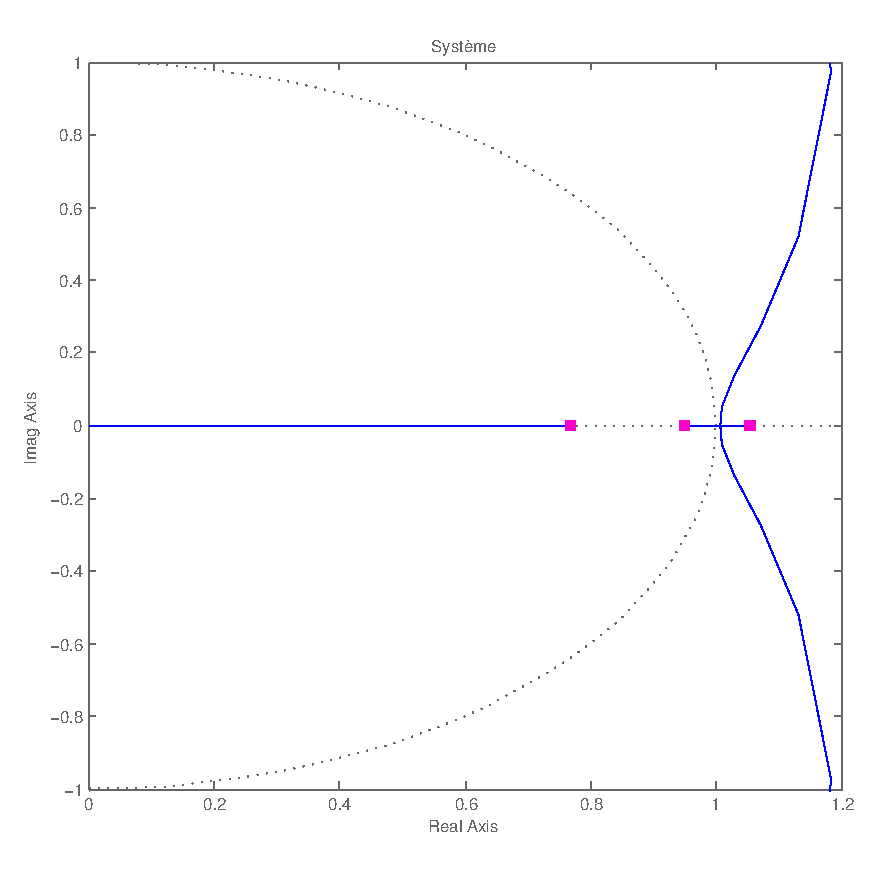
\includegraphics[scale=0.50]{RLN_Sys_Seul.pdf}
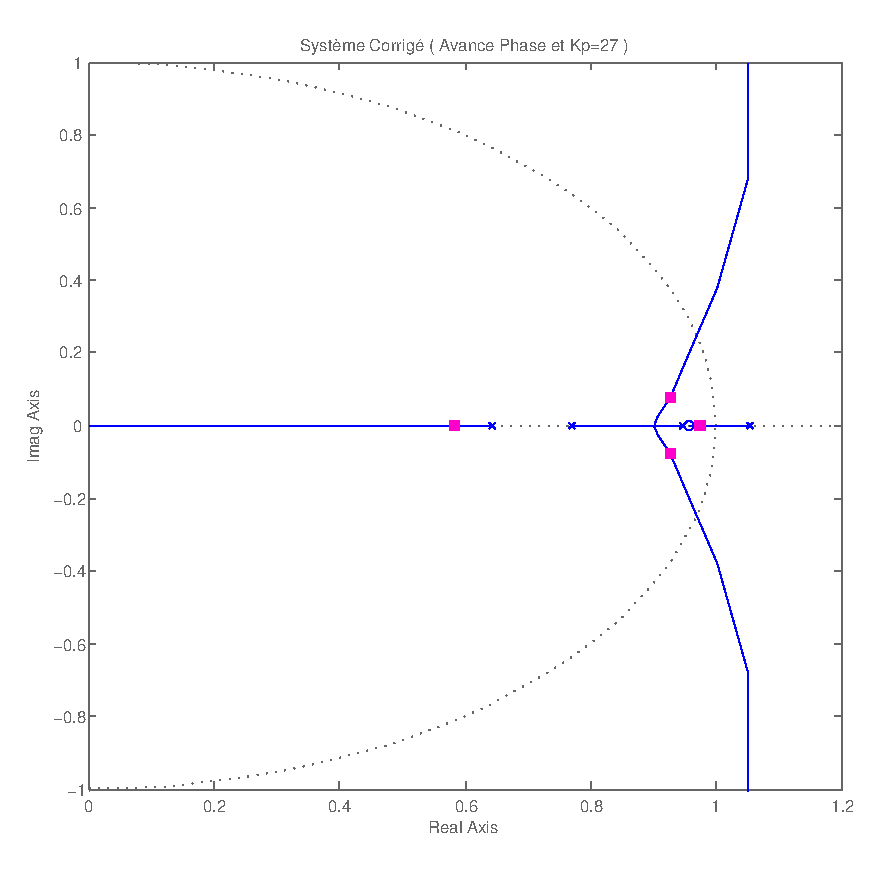
\includegraphics[scale=0.50]{RLN_Sys_AvPh_K27.pdf}

\section{Conclusion}

Grâce à cette étude, nous avons pu trouver des valeurs de paramètres de correcteurs qui nous permettent de stabiliser le système. Cependant, nous pouvons nous interroger sur la fiabilité de ces paramètres étant donné qu'ils sont basés sur une approximation linéaire du système. De même, le modèle du champ magnétique pourrait se révéler trop imprécis et ainsi fausser le calcul des constantes. Il faudra donc garder cela à l'esprit pour éventuellement réévaluer nos paramètres par la suite. 

\end{document}
